\documentclass[10pt]{article}
\usepackage[polish]{babel}
\usepackage[utf8]{inputenc}
\usepackage[T1]{fontenc}
\usepackage{amsmath}
\usepackage{amsfonts}
\usepackage{amssymb}
\usepackage[version=4]{mhchem}
\usepackage{stmaryrd}
\usepackage{graphicx}
\usepackage[export]{adjustbox}
\graphicspath{ {./images/} }

\title{LIGA MATEMATYCZNA \\
 PÓŁFINAE 5 lutego 2010 \\
 GIMNAZJUM }

\author{}
\date{}


\begin{document}
\maketitle
\section*{ZADANIE 1.}
Czy liczba \(\sqrt{16+8 \sqrt{3}}-\sqrt{16-8 \sqrt{3}}\) jest całkowita? Odpowiedź uzasadnij.

\section*{ZADANIE 2.}
W auli odbyło się zebranie ucznión klas pierwszych dotyczace wyboru języków obcych. Każdy uczeń wybrał co najmniej jeden język i nie więcej niż dwa. 50 uczniów chce uczyć się języka angielskiego, 25 języka niemieckiego, 13 języka francuskiego i 5 jęzka włoskiego. Żaden z uczniów chcących uczyć się języka włoskiego nie chce uczyć się innego języka. 15 uczniów spośród chcących uczyć się języka angielskiego chce uczyć się też języka niemieckiego, a 3 języka francuskiego. Tylko jeden uczeń zamierza uczyć się języka niemieckiego i języka francuskiego. Ilu uczniów było na tym spotkaniu?

\section*{ZADANIE 3.}
Rozwiąż układ równań

\[
\left\{\begin{array}{l}
x(x+y+z)=2 \\
y(x+y+z)=4 \\
z(x+y+z)=10
\end{array}\right.
\]

\section*{ZADANIE 4.}
Wyznacz liczbę naturalną \(n\), która jest podzielna przez 16 i ma 9 mniejszych od siebie dzielników, których suma równa się \(n\).

\section*{ZADANIE 5.}
Punkty \(E, F, G, H\) dzielą boki prostokąta \(A B C D\) w stosunku 1:2. Jaki jest stosunek pola czworokąta \(E F G H\) do pola prostokąta \(A B C D\) ?\\
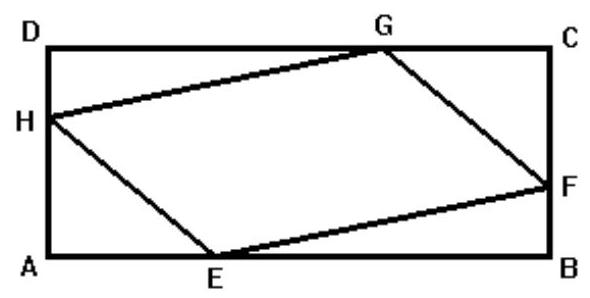
\includegraphics[max width=\textwidth, center]{2024_11_21_b04ca9863e497de14b4bg-1}


\end{document}